\section{Block persistence}
The blocks in the chain have to be persisted to be usable over a prolonged time.
There are several design goals to be achieved in the way that the blocks are persisted:
\begin{itemize}
    \item Availlability
    \item Queryable
    \item Resilient
\end{itemize}

The blocks have to be readily available.
Any block can be needed at any time to verify a reputation claim
or to be distributed to another peer on request.
The blocks do have the property that they are likely to be needed sequentially.
Blocks that were never known at some point by the node are ignored for this design goal
and are treated separately.
\todo{Were are they discussed?}

Information is stored into the blocks and this information should be queryable in a easy way.
Making the information queryable makes the information accessible
and allows to perform analysis of the chain.
For example the a chain has to be analysed to verify it is correct.

If parts of the chain or the whole chain are lost due to failure,
then the node will lose its reputation.
This is clearly unacceptable and the persistence should be resilient against failure
and prevent loss.
The chain will be persistent across system shutdown,
but should also provide ways of preventing loss in case of hardware failure.

\subsection{SQLite}
SQLite is a relational database and provides simple bindings to use in Python\cite{owens-sqlite}.
It implements SQL and is ACID-compliant\cite{haerder-ACID}.
SQLite saves its database to a single file on disk and provides local storage.
It does not use the typical client-server architecture seen in most other database systems
and the code is directly linked in the program itself.
A separated process is not used to run SQLite.

Tribler uses SQLite to persist its data to disk.
Because Tribler already provides integration and uses SQLite,
SQLite was chosen to be used to persist the blocks.
SQLite adequately meets the design goals needed for the persistence layer of MultiChain.

The data in the SQLite database is readily available.
Queries can be executed directly by the code.
Latency is reduced because there is not another process or server that needs to be contacted.
Concurrency is handled by the SQLite library,
but Dispersy is single threaded so this is not a problem.

Information stored in a SQLite database is inserted and retrieved using SQL\cite{date-sql}.
SQL allows easy information retrieval and can be used to retrieve specific information.
Using SQL information can easily be retrieved that is necessary to verify the chain.

ACID-compliance guarantees that transactions are comitted reliably.
The database is stored locally on hard disk.
This is done in a single file and has no redundant backups by default.
The operator of the node will be responsible to make backups,
but this is trivial for a single file.
The file can be used by any SQLite library on any computer.
To completely resume operations on a different computer
additional functionality is required to export and import private keys of the MultiChain community.

\subsection{Persistence layer}
A persistence layer is added to the MultiChain community
that provides all functionality to persist blocks and query blocks.
This layer extends and uses functionality of the Database class in Dispersy.
An overview of the layering in the software architecture can be seen in Figure \ref{fig:persistence-layer}.

\begin{figure}
	\centerline{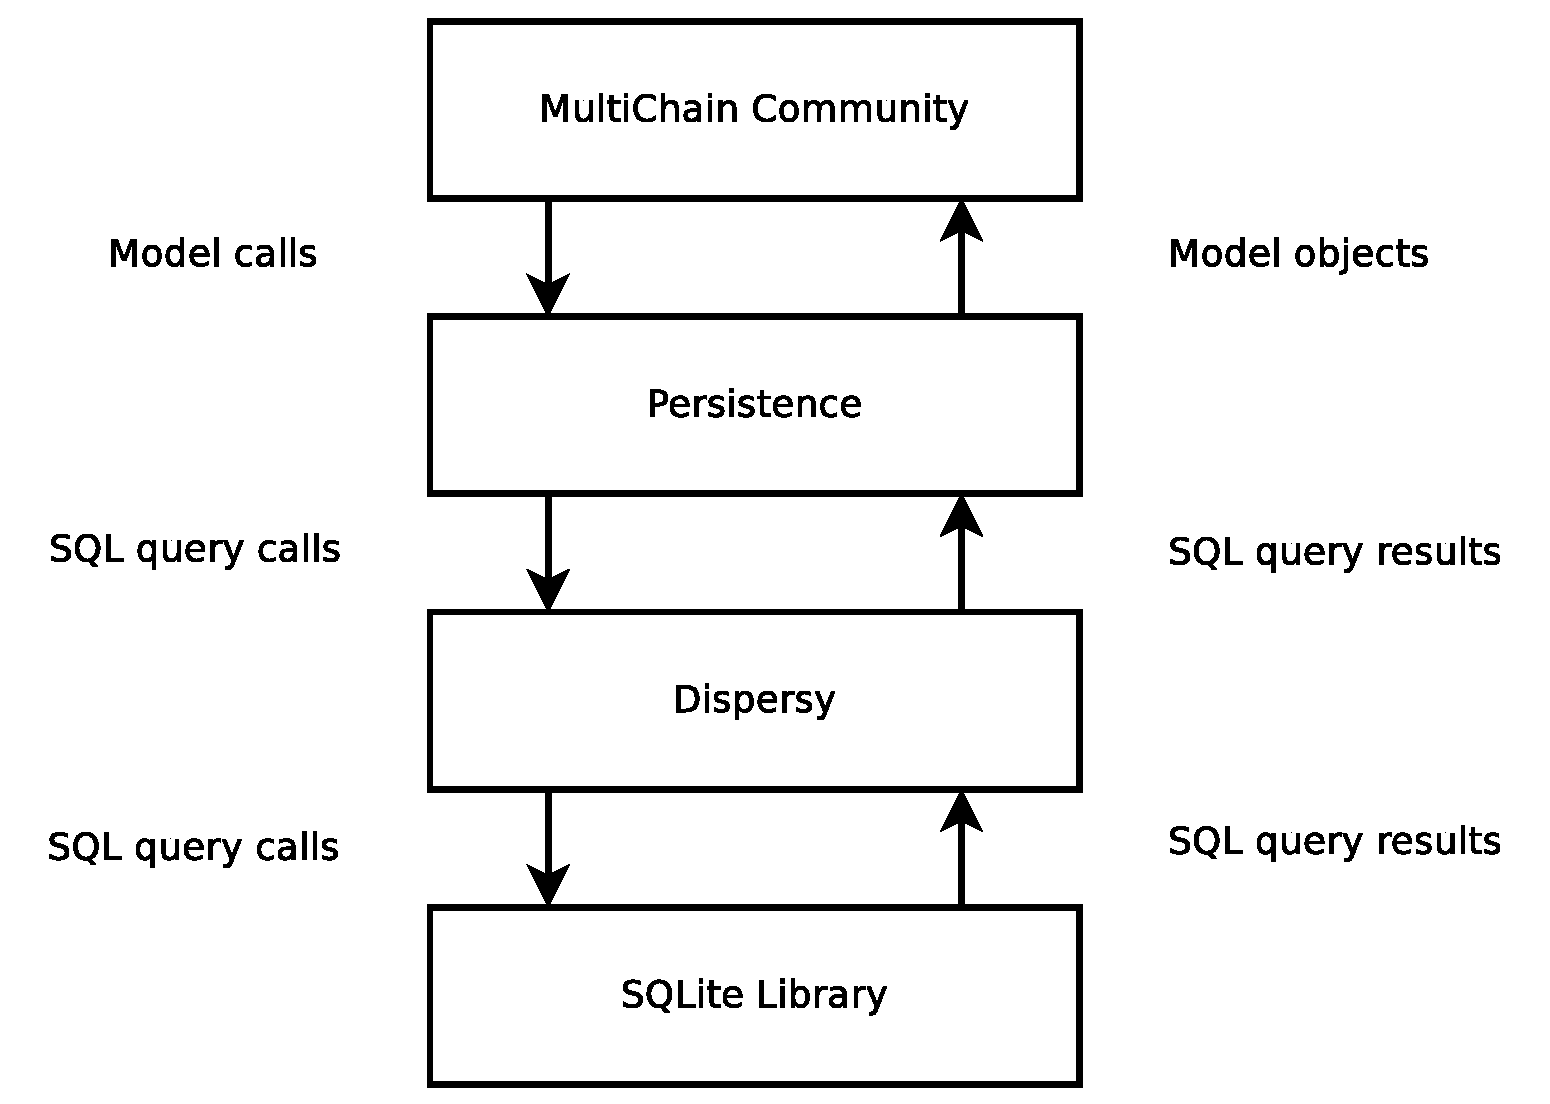
\includegraphics[scale=0.3]{design/figs/persistence-layer.eps}}
	\caption{Persistence layering in the software architecture}
	\label{fig:persistence-layer}
\end{figure}

The MultiChain Community calls functions in the persistence layer that have implicit knowledge about the model.
The Persistence layer formats SQL queries and passes these to the Dispersy layer.
The Dispersy layer performs several sanitation checks and passes these queries to the SQLite Library.
The SQLite Library and Dispersy layer both return the result of the SQL query.
These results are transformed by the Persistence layer into objects of the model usable by the MultiChain Community.

The only information that is saved are blocks.
The information all fits within one table.
A single block is saved as a single record called a row in a relation database.
Every attribute of a block is a single column in the row.
All attributes are saved directly into the database,
except for the public keys.
These public keys are hashed and these hashes are used as an identifier, called mid, in Dispersy.
The public keys are already saved in the Dispersy database.
When a block is retrieved from the database the public key is retrieved from Dispersy using the mid.
An overview of every attribute and the size of the attribute inside the database can be seen in Table \ref{table:block_size_persistence}.
SQLite can grow the size of integers in its database to fit the required size
and therefore it can be in the range of $1,2,3,4$ bytes.

\begin{table}[]
\begin{adjustwidth}{-.5in}{-.5in}
\begin{center}
\begin{tabular}{lll||lll}
Name              & Type             & Bytes                  & Name              & Type             & Bytes    \\ \hline
Uploaded MBytes   & unsigned integer & 1,2,4                  & Downloaded MBytes & unsigned integer & 1,2,4    \\
Total Up A        & unsigned integer & 1,2,4,8                & Total Up B        & unsigned integer & 1,2,4,8  \\
Total Down A      & unsigned integer & 1,2,4,8                & Total Down B      & unsigned integer & 1,2,4,8  \\
Prior Record A    & SHA1 digest      & 20                     & Prior Record B    & SHA1 digest      & 20       \\
Sequence Number A & signed integer   & 4                      & Sequence Number B & signed integer   & 4        \\
Mid A             & SHA1 digest      & 20                     & Mid B             & SHA1 digest      & 20       \\
Signature A       & EC signature     & 40                     & Signature B       & EC signature     & 40
\end{tabular}
\caption{Block size inside the database.}
\label{table:block_size_persistence}
\end{center}
\end{adjustwidth}
\end{table}

Every attribute is queryable in the database.
A public key can be converted to mid and is searched this way.
Every attribute is queryable to make the system  extensible
and usable when the next incremental steps are implemented.
It is presently unknown what information precisly will be needed,
so every information is now made available for the future.

\subsection{Upper limit uploaded and downloaded MB}
The maximum integer size of the total up and total down impose an upper limit
on the total uploaded and downloaded MB that MultiChain can track.
This limit is imposed by SQLite and is $2^{62}$.
Bigger numbers cannot be saved in SQLite using a native datatype.
The upper limit for MultiChain is therefore $4.612 * 10^9$\todo{ask about *} petabytes.
This is clearly more than sufficient.

\subsection{Dispersy database}
Dispersy keeps track of information on its own.
A record is kept of any message that can be retrieved using a message id.
The message is saved in a converted format and will be decoded when the message is retrieved.

Instead of storing information in a separate database,
the information could have been retrieved from the Dispersy database.
But the Dispersy database is not queryable.
All the information is stored in a converted format
that prevents queries to search the message for its contents.
For this reason, the dispersy database is not used and a separate database is used.

A future, possible improvement to Dispersy would be to save messages queryable in its database.
This would eliminate the current need for separate databases that contain aggregrated information.
The information is stored in two places within Tribler and this could be eliminated.
It would reduce the disk footprint and the amount of read/write transactions
as only one database would have to be maintained.
The I/O ineractions are a problem according to Tribler maintainers.